\documentclass[E:/Latex/ExtraWork/ComputerArchitechture/Report.tex]{subfiles}
\usepackage[utf8]{inputenc}
\PassOptionsToPackage{english, british}{babel}
\usepackage[english, british]{babel}
\usepackage{graphicx}
\graphicspath{{../ComputerArchitechture/Chapter2/Figure/}}
\usepackage{amsmath}
\usepackage{amsfonts}
\usepackage{multirow}
\usepackage{booktabs}
\usepackage{indentfirst}
\usepackage{tabularx}
\usepackage{amssymb}
\usepackage{setspace}		%use \doublespacing
\begin{document}
	\begin{otherlanguage}{english}
		\chapter{Thiết kế CPU RICSV 32 đơn chu kỳ}
			\section{Thiết kế phần cứng}
				\textbf {Phần cứng được thiết kế theo sơ đồ sau:}
					\begin{figure}[h!]
						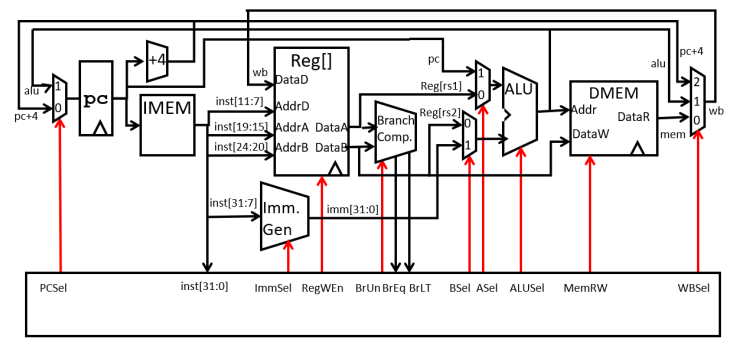
\includegraphics[scale = 0.9]{Figure/Fig1.png}
						\centering
					\end{figure}


				\textbf {Trong đó, các tín hiệu kết nối được đặt tên theo bảng sau:}
				\begin{table}[!ht]
				\begin{tabular}{|l|l|l|l|}
				\hline
				\textbf{Name}           & \textbf{Khối bắt đầu} & \textbf{Khối đích}                                                   & \textbf{Ý nghĩa}                                                             \\ \hline
				\textbf{clk}            & Input của CPU         & \begin{tabular}[c]{@{}l@{}}PC, Register bank,\\ DMEM\end{tabular}    & \begin{tabular}[c]{@{}l@{}}Xung clock điều khiển \\ chu kỳ lệnh\end{tabular} \\ \hline
				\textbf{pc\_in}         & PCmux                 & PC                                                                   & PC của lệnh tiếp theo                                                        \\ \hline
				\textbf{pc\_out}        & PC                    & \begin{tabular}[c]{@{}l@{}}IMEM, PC+4, \\ ALUmux1\end{tabular}       & PC hiện tại                                                                  \\ \hline
				\textbf{pc\_plus4\_out} & PC+4                  & PCmux                                                                & PC\textless{}-PC+4                                                           \\ \hline
				\textbf{rs1}            & IMEM                  & Register Bank                                                        & Địa chỉ của rs1                                                              \\ \hline
				\textbf{rs2}            & IMEM                  & Register Bank                                                        & Địa chỉ của rs2                                                              \\ \hline
				\textbf{rd}             & IMEM                  & Register Bank                                                        & Địa chỉ của rd                                                               \\ \hline
				\textbf{rs1\_out}       & Register Bank         & \begin{tabular}[c]{@{}l@{}}BranchComp, \\ ALUmux1\end{tabular}       & Data của rs1                                                                 \\ \hline
				\textbf{rs2\_out}       & Register Bank         & \begin{tabular}[c]{@{}l@{}}BranchComp, ALUmux2, \\ DMEM\end{tabular} & Data của rs2                                                                 \\ \hline
				\textbf{imm\_in}        & IMEM                  & ImmGen                                                               & Data vào ImmGen                                                              \\ \hline
				\textbf{imm\_out}       & ImmGen                & ALUmux2                                                              & \begin{tabular}[c]{@{}l@{}}Data sau khi qua \\ khối ImmGen\end{tabular}      \\ \hline
				\textbf{alumux1\_out}   & ALUmux1               & ALU                                                                  & Toán hạng 1 vào ALU                                                          \\ \hline
				\textbf{alumux2\_out}   & ALUmux2               & ALU                                                                  & Toán hạng 2 vào ALU                                                          \\ \hline
				\textbf{aluout}         & ALU                   & \begin{tabular}[c]{@{}l@{}}DMEM, Wbmux, \\ PCmux\end{tabular}        & Ngõ ra của ALU                                                               \\ \hline
				\textbf{dmem\_out}      & DMEM                  & Wbmux                                                                & Data đọc của DMEM                                                            \\ \hline
				\textbf{wb\_out}        & Wbmux                 & Register Bank                                                        & Data ghi ngược                                                               \\ \hline
				\end{tabular}
				\end{table}

				\newpage
				\textbf {Thiết kế khối Control}
				
				Tiến hành lập bảng bao gồm các lệnh, các tín hiệu vào và tín hiệu ra, sau đó phân tích từng lệnh vè điền vào bảng như hình sau:
					\begin{figure}[h!]
						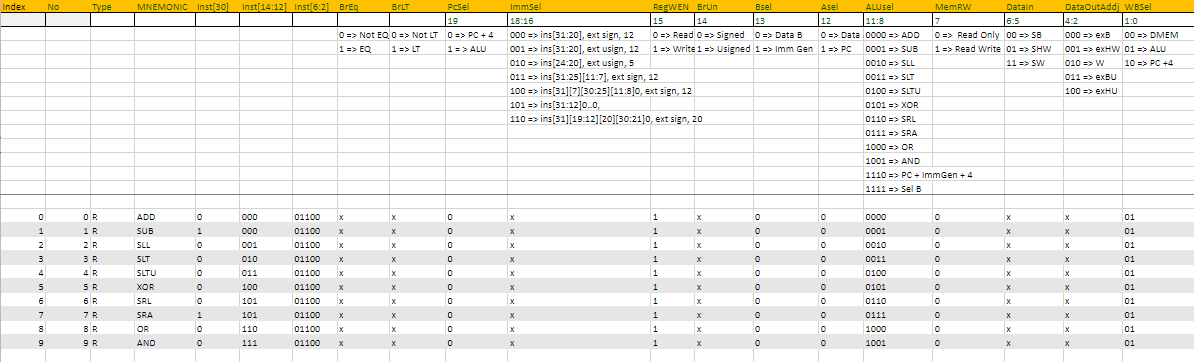
\includegraphics[scale = 0.6]{Figure/Fig2.png}
						\centering
					\end{figure}

				Sau đó, chuyển bảng vừa lập thành khối Control. Viết theo kiểu ROM

				\textbf {Thiết kế các khối chức năng }
				
				Phân tích từng khối: chức năng, ngõ vào, ngõ ra và viết riêng từng module.

				\newpage
				\section{Thực hiện mô phỏng}
				\subsection{Viết đoạn chương trình test}
				\begin{itemize}
					\item Lấy 10 số lưu trong DMEM và sắp xếp lại rồi lưu vào DMEM ở 10 vị trí tiếp theo.
					\item Tính giai thừa số lớn nhất và lưu ở vị trí tiếp theo.
					\item Tính số Fibonanci của số lớn nhất và lưu ở vị trí tiếp theo.
				\end{itemize}
				\subsection{Test dạng sóng trên ModelSim và kết quả mô phỏng}
				
				Kết quả sau khi chạy đoạn code trên: 
					\begin{figure}[h!]
						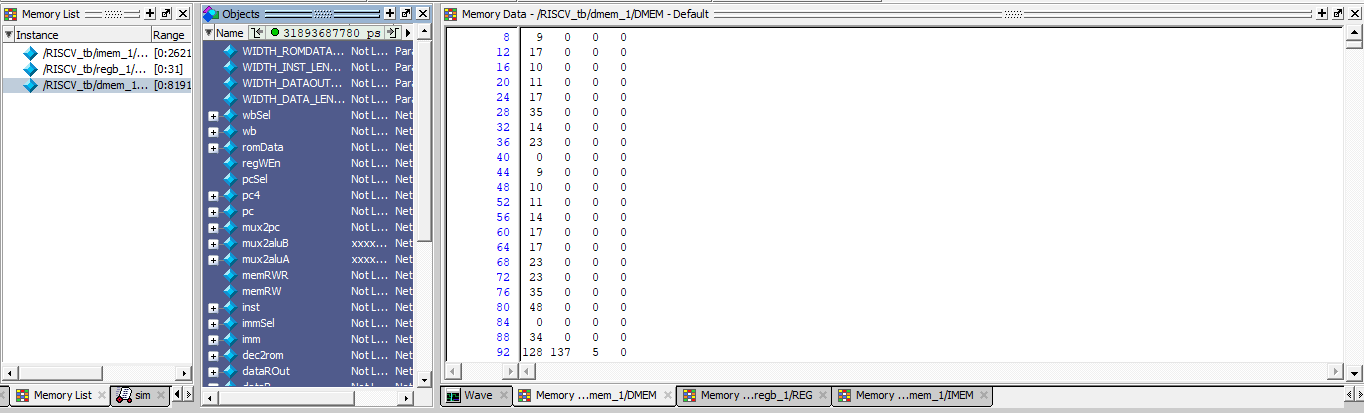
\includegraphics[scale = 0.5]{Figure/Fig3.png}
						\centering
					\end{figure}

				Dạng sóng của đoạn code trên:
					\begin{figure}[h!]
						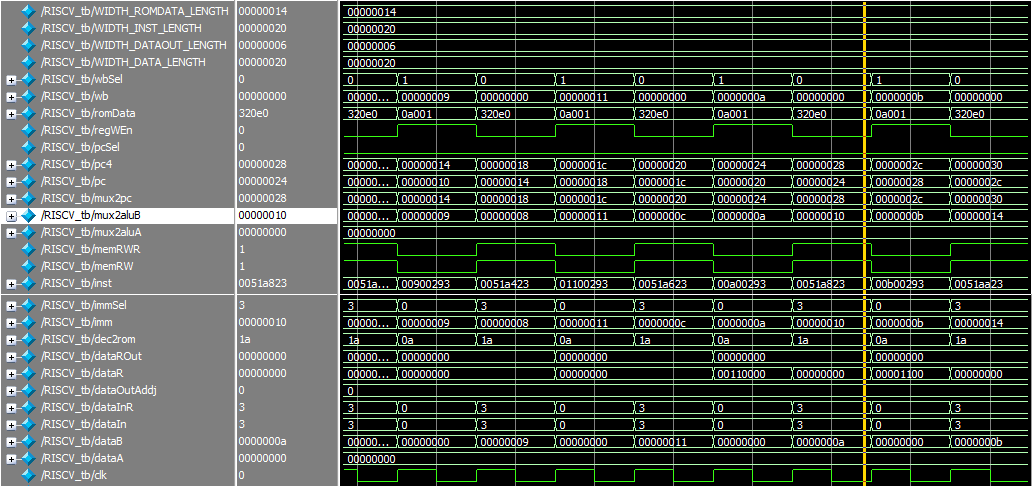
\includegraphics[scale = 0.6]{Figure/Fig6.png}
						\centering
					\end{figure}

				\newpage
				Kết quả mô phỏng của khối ALU:
					\begin{figure}[h!]
						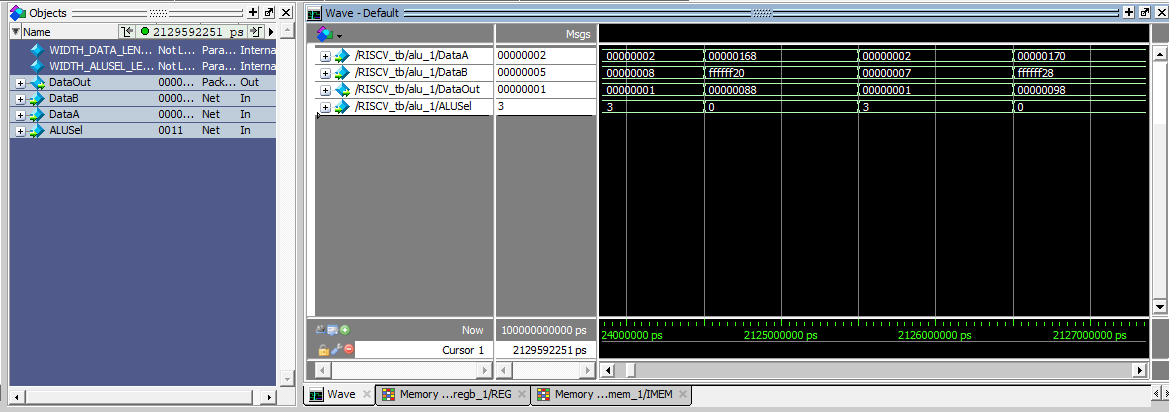
\includegraphics[scale = 0.6]{Figure/Fig4.png}
						\centering
					\end{figure}
				
				Kết quả mô phỏng khối Branch Comp:
					\begin{figure}[h!]
						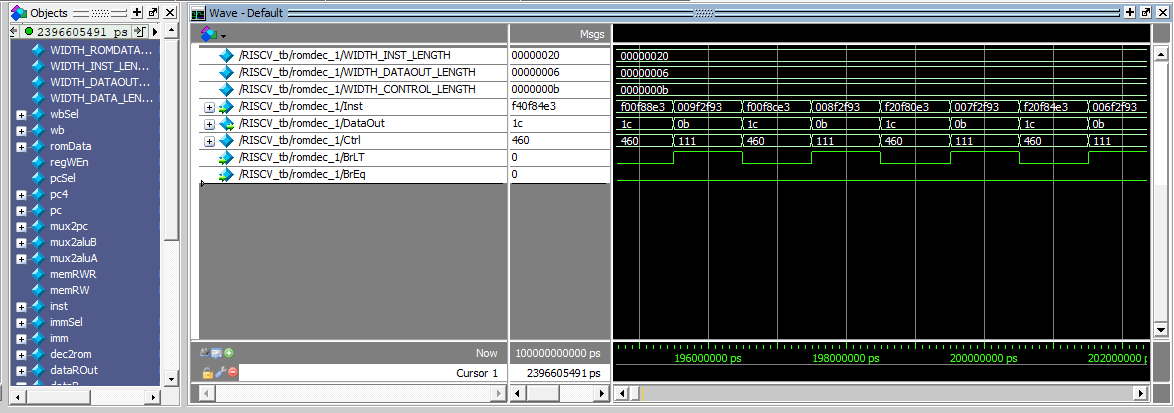
\includegraphics[scale = 0.6]{Figure/Fig5.png}
						\centering
					\end{figure}

				Kết quả mô phỏng khối DMEM:
					\begin{figure}[h!]
						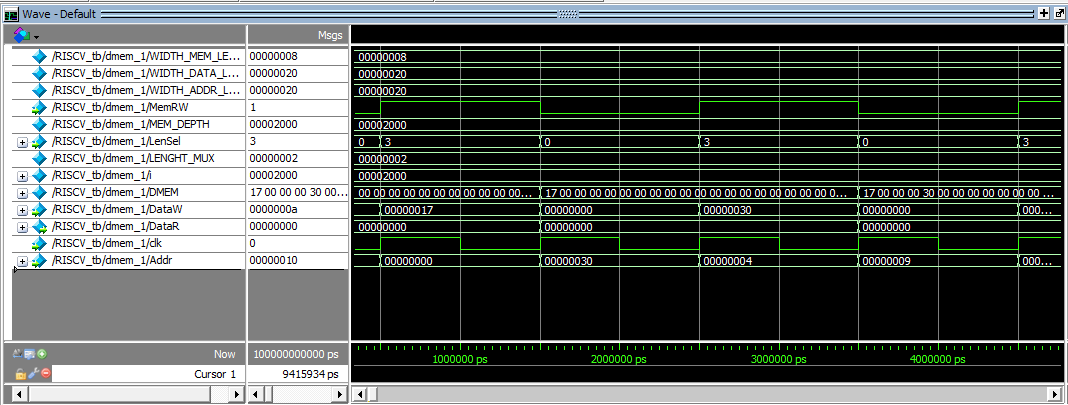
\includegraphics[scale = 0.6]{Figure/Fig7.png}
						\centering
					\end{figure}

				\newpage
				Kết quả mô phỏng khối Reg:
					\begin{figure}[h!]
						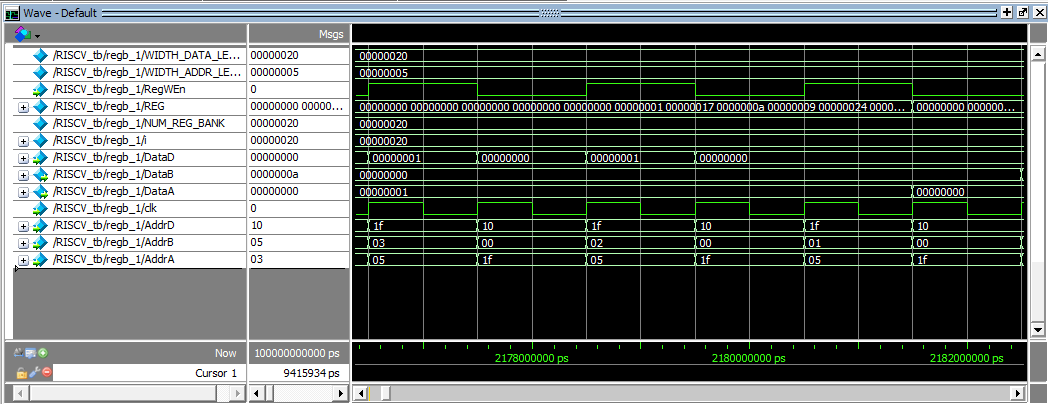
\includegraphics[scale = 0.6]{Figure/Fig8.png}
						\centering
					\end{figure}

				Kết quả mô phỏng khối Imm:
					\begin{figure}[h!]
						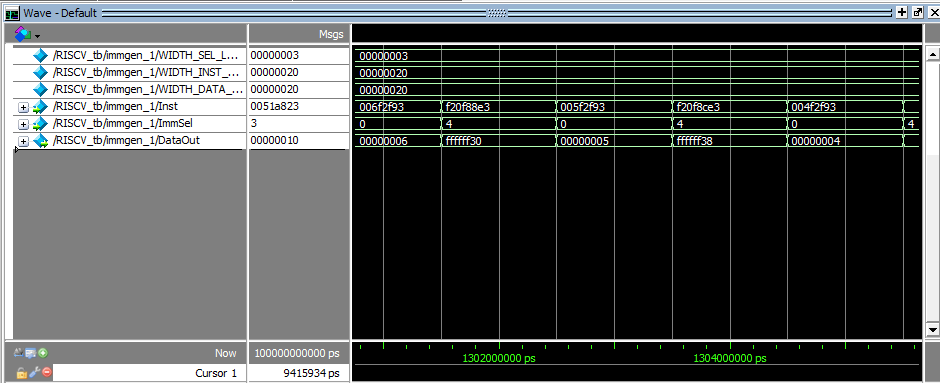
\includegraphics[scale = 0.7]{Figure/Fig9.png}
						\centering
					\end{figure}

	\end{otherlanguage}

\end{document}